\section{Projekce}

\subsection{Věta o nejlepší aproximaci}
Je-li $C \subseteq \R^n$ neprázdná uzavřená konvexní množina, pak pro každé $x \in \R^n$ existuje právě jeden bod 
$\hat y \in C$ tak, že $\dist (x; C) = ||x-\hat y||$.

Důkaz.

(a) Existence\\
Cíl: Existuje bod minima\\
Úvaha:
\begin{multicols}{2}

    \begin{tikzpicture}[fill=gray]
        \begin{scope}
            \clip (0,0) circle (2);
            \clip (3,0) circle (2);
            \fill[pattern=north east lines] (0,0) circle (2);
        \end{scope}
        
        \draw (0,0) circle (2) node [text=black] {$M$};
        \draw (3,0) circle (2);
    
        \filldraw[black] (1, 0) circle (2pt) node[left] {$z$};
        \filldraw[black] (2, 0) circle (2pt) node[right] {$y$};
        \filldraw[black] (3, 0) circle (2pt) node[right] {$x$};
    
        \draw[->, thick] (1,-2.5) -- (1.5,-1) node[midway, above, sloped] {$C_z \not= \emptyset$}; % TODO upravit sipku
    \end{tikzpicture}

    \begin{adjustwidth}{-2em}{0pt}
        $M$ je obecná konvexní množina.

        $R = ||x-z||$,

        $Cz = M \cap B (x, R) = M \cap \bc{a \in \R^n \mid \|z-a\| \leq R}$.\\
        $\uparrow$\\
        $\underbrace{\text{uzavřená, omezená}}_\text{kompaktní}$, neprázdná

        Tedy $a \mapsto ||x-a||$ je spojitá.

        $\Rightarrow$ Spojitost na kompaktní množině znamená, že $f$ nabývá na $C_z$ minima dle 
        \href{https://cs.wikipedia.org/wiki/Weierstrassova_v%C4%9Bta}{Weierstrassovy věty}.
    \end{adjustwidth}
\end{multicols}
Ať $y$ je bod minima. Všechny body v $M$ mají od $x$ vzdálenost $\geq ||x-y||. \qed$

(b) Jednoznačnost.\\
Cíl: Pokud $a,b \in \R^n : ||x-a|| = ||x-b|| = \overbrace{\dist(x,M)}^\delta$, pak $a=b$.\\
Lemma, rovnoběžníkové pravidlo: $u,v \in \R^n \Rightarrow ||u+v||^2 + ||u-v||^2 = 2\left(||u||^2 + ||v||^2\right)$.\\
Důkaz lemma: 
\[
    ||u+v||^2 + ||u-v||^2 = \langle u+v, u+v \rangle + \langle u-v, u-v \rangle = ||u||^2 + 2 \langle u, v \rangle + 
    ||v||^2 + ||u||^2 - 2 \langle u, v \rangle + ||v||^2
\] 
\[
    = 2\left( ||u||^2 + ||v||^2 \right) \text{.} \qed
\]
Důkaz jednoznačnosti:\\
Ať $y = \frac{1}{2}a + \frac{1}{2}b$. \\
Pak $\delta^2 \leq ||x-y||^2 = ||x-\frac{1}{2}a - \frac{1}{2}b||^2 = ||\frac{1}{2}(x-a) + \frac{1}{2}(x-b)||^2 = 
\frac{1}{4}||\underbrace{(x-a)}_{u} + \underbrace{(x-b)}_{v}||^2 \\ 
\stackrel{\text{lemma}}{=} \frac{1}{4} \left[ 2 \left(\underbrace{||x-a||^2}_{\delta^2} + \underbrace{||x-b||^2}_{\delta^2}\right) 
- \underbrace{||(x-a) + (x-b)||^2}_{b-a}\right] = \delta^2 - \frac{1}{4} ||b-a||^2 \Rightarrow \delta^2 \leq \delta^2 - 
\underbrace{\frac{1}{4} ||b-a||^2}_{\leq 0 \Rightarrow a=b} \text{.}$

\subsection{Projekce bodu a variační nerovnost}\label{varNer}
Nechť $C \subseteq \R^n$ je neprázdná uzavřená konvexní množina, $x \in \R^n$ a $y \in C$. Pak následující tvrzení jsou
ekvivalentní:
\begin{enumerate}[(1)]
    \item $y = P_C (x)$, kde $P_C(x)$ je projekční operátor.
    \item Pro každé $z \in C$ je $\langle x-y, z-y \rangle \leq 0$. 
\end{enumerate}

Důkaz.

$(1) \Rightarrow (2)$:\\
Ať $v_\lambda = y + \lambda(z-y)$, $\lambda \in (0,1]$.\\
Pak
\[
    ||x-y||^2 \leq ||x-v_\lambda||^2 = ||x-y-\lambda(z-y)||^2 = \langle (x-y) - \lambda(z-y), (x-y) - \lambda(z-y)\rangle 
\]
\[
    ||x-y||^2 \leq ||x-y||^2 - 2 \lambda \langle x-y, z-y\rangle + \lambda^2 ||z-y||^2
\]
\[
    \Rightarrow \langle x-y, z-y\rangle \leq \frac{\lambda}{2} ||z-y||^2 \rightarrow 0 \text{ pro } \lambda \rightarrow 0^+
\]
\[
    \Rightarrow \langle x-y, z-y\rangle \leq 0 \text{.} \qed
\]

$(2) \Rightarrow (1)$:\\
Ať $z \in C$.\\
Pak
\[
    0 \geq \langle x-y, z-y \rangle = \langle x-y, (z-x)+(x-y) \rangle = \langle x-y, z-y \rangle + ||x-y||^2  
\]
\[
    \langle x-y, z-y \rangle + ||x-y||^2 \geq  ||x-y||^2 - \underbrace{|\langle x-y, z-y\rangle|}_{\text{odhad shora}} \geq \star
\]
\[
    \star = ||x-y||^2 - ||x-y|| \cdot ||z-x||.
\]
Je-li $x \not= y$, pak vydělíme: $||z-x|| \geq ||x-y||$.\\
Je-li $x=y$, pak $y \in C : x \in C \dots$ triviální. $\qed$ 

\subsection{Koule?} %TODO: co se tady počítá?


\subsection{Věta o ortogonálním rozkladu} \label{ortoRoz}

Nechť $L \subseteq \R^n$ je lineární podprostor. Potom platí:

\begin{enumerate}[(a)]
    \item $P_L : \R^n \rightarrow \R^n$ je lineární zobrazení.
    \item Pro každé $x \in \R^n$ je $P_{L^\perp} (x) = x - P_L (x)$.
    \item Pro každé $x \in \R^n$ existují jednoznačně určené body $y \in L$ a $z \in L^\perp$ tak, že $x=y + z$. Navíc 
    $y = P_L(x)$ a $z=P_{L^ \perp} (x)$.
\end{enumerate}

Důkaz.

(a)\\
Cíl: Dokázat vlastnosti lineárního zobrazení, tedy 
\begin{enumerate}
    \item $P_L (\alpha x) = \alpha \cdot P_L (x), \forall \alpha \in \R, x \in \R^n$.
    \item $P_L (x + y) =   P_L (x) +  P_L (y), \forall x,y \in \R^n$.
\end{enumerate}

1. : Ať $z \in L$.
Pak 
\[
    \langle \alpha x - \alpha P_L (x), z - \alpha P_L (x) \rangle = \alpha  \langle x - P_L (x), z - \alpha P_L (x)\rangle
\]
\[
    \stackrel{\alpha \not= 0}{=} \underbrace{\alpha^2}_{> 0} \langle x - P_L (x), \underbrace{\frac{1}{\alpha} 
    \cdot z}_{\in L} - P_L (x)\rangle
\]
Tedy $P_L(\alpha x) = \alpha P_L(x), \forall \alpha \not= 0$. Pro $\alpha =0$ zřejmě plyne z lineárnosti zobrazení.

2. : Ať $z \in L$.

\[
    \langle \underbrace{x + y - (P_L(x) + P_L(y))}_{(x-P_L(x)) + (y - P_L(y))}, z - (P_L (x) + P_L(y)) \rangle
\]
\[
    \underbrace{\langle x - P_L(x), \underbrace{(z - P_L(y))}_{\in L} - P_L(x)\rangle}_{\leq 0} + 
    \underbrace{\langle y - P_L(y), \underbrace{(z - P_L(x))}_{\in L}  - P_L (y)\rangle}_{\leq 0} \leq 0.
\]

Z \hyperref[varNer]{variační nerovnosti} tedy plyne, že $P_L$ je nutně lineární. $\qed$

\begin{multicols}{2}
    (b) Pro každé $x \in \R^n$ je $P_{L^\perp} (x) = x - P_L (x)$.

    L $\dots$ lineární podprostor $\R^n$,\\
    $L^\perp = \bc{x \in \R^n \mid \langle x, y\rangle = 0, \forall y \in L}$.

    Důkaz.\\
    Cíl: $P_{L^\perp} (x) = x - P_L(x)$.\\
    Ať $x \in \R^n, z \in L^\perp$. Pak

\columnbreak

    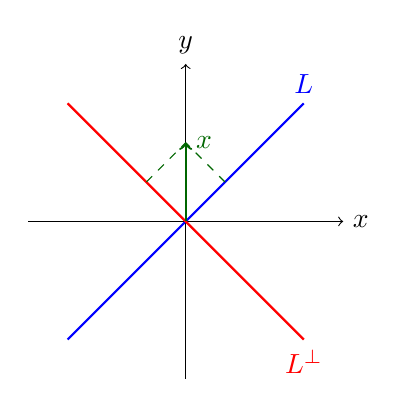
\begin{tikzpicture}
        \draw[->] (-2,0) -- (2,0) node[right] {\(x\)};
        \draw[->] (0,-2) -- (0,2) node[above] {\(y\)};
        
        \draw[blue, thick] (-1.5,-1.5) -- (1.5,1.5) node[above] {\(L\)};
        \draw[red, thick] (-1.5,1.5) -- (1.5,-1.5) node[below] {\(L^\perp\)};

        \draw[black!60!green, dashed] (0.5,0.5) -- (0,1);
        \draw[black!60!green, dashed] (-0.5,0.5) -- (0,1);
        \draw[->][black!60!green, thick] (0,0) -- (0,1) node[right] {$x$};
    \end{tikzpicture}
\end{multicols}

\[
    \langle x - (x - P_L(x)), z - (x - P_L(x))\rangle = \langle \underbrace{P_L(x)}_{\in L}, z - (x - P_L(x))\rangle
\]
\[
    = \underbrace{\langle P_L (x), z\rangle}_0 - \langle P_L (x), x-P_L(x)\rangle = \langle x - P_L (x), 0 - P_L(x)\rangle \leq 0. \qed
\]
% TODO: doplnit zdůvodnění

(c) Pro každé $x \in \R^n$ existují jednoznačně určené body $y \in L$ a $z \in L^\perp$ tak, že $x=y + z$. Navíc 
$y = P_L(x)$ a $z=P_{L^ \perp} (x)$.

Ať $x \in \R^n$.

Důkaz existence.\\
Pak  $x = \underbrace{P_L (x)}_{\in L} + \underbrace{(x - P_L (x))}_{\in L^\perp}. \qed$

Důkaz jednoznačnosti.\\
Ať $a \in L, b \in L^\perp$ takové, že $x = a+b$.\\
Cíl: $a = P_L (x)$

Ať $z \in L$.
\[
    \langle x-a, z-a\rangle = \langle b, \underbrace{z-a}_{\in L}\rangle = 0 \leq 0 \implies a = P_L (x) \implies 
    x - P_L(x) = b \stackrel{\hyperref[varNer]{(2)}}{\implies} P_{L^\perp} (x) = b. \qed
\]